%%---------------Chapter 5------------------------------
\chapter{Metabolic Modelling with Hybrid Automata}\label{chap:model}

\subsection{Formulation of a Reference Model}

%While the modeling approach that follows is applicable to any microbe with known stoichiometry, it has been developed with a specific reference co-culture in mind. This co-culture consists of two microorganisms that possesses emergent metabolic capacity when placed in the same \textit{in silico} environment, given that the simulated medium contains necessary levels of essential nutrients. Both organisms have simple metabolic networks that can be easily visualized and understood without computational analysis. This reference model is useful because it represents the elementary case where emergent metabolism can be generated by microbe interaction. Furthermore, the \textit{in silico} process for emergent metabolite detection can still be carried out using the simple model organisms and further honed to make the approach more useful for a realistic bioengineering scenario.
The model organisms presented in Chiu et al.'s detection procedure for emergent metabolism \cite{Chiu14} directly provide the stoichiometry, bounds, and dynamics for the reference microbes in this work. Chiu's work gives a) a highly granular description of the dFBA procedure used to detect emergent metabolites, including parameters of simulation, and b) a detailed analysis (with visualizations) of the expected qualitative behavior. Thus, Chiu's work serves as an an excellent launchpad for any further investigation of emergent metabolism on the cellular level -- it gives input models with a set of simulation results to validate against a new approach.

The microorganism models, which shall be denoted Organism 1 and Organism 2, are defined as follows:

%In this model co-culture, the environmental shift induced by one organism promotes a second organism to activate an alternative pathway and consequently secrete an emergent metabolite.

\textbf{Organism 1:}
The internal stoichiometric matrix contains the reaction stoichiometries for intracellular metabolites, all of which exhibit steady-state behavior, whereas the uptake and secretion stoichiometric matrix shows the reaction stoichiometries for external metabolites in the growth medium.

\begin{tabularx}{\textwidth}{l}
  \textbf{Internal Stoichiometric Matrix} \\

$\begin{bmatrix}
\_ & R_1 & R_2 & R_3 & R_4 & J_1 & J_2 & J_3 & J_4 \\
\frac{dA}{dt} & -1 & 0 & 0 & 0 & -1 & 0 & 0 & 0 \\
\frac{dD}{dt} & 1 & -3 & 0 & -1 & 0 & 0 & 0 & 0 \\
\frac{dZ}{dt} & 0 & 1 & -10 & 1 & 0 & 0 & 0 & 0 \\
\frac{dW}{dt} & 0 & 2 & 0 & 0 & 0 & 0 & 0 & -1 \\
\frac{dC}{dt} & 0 & 0 & 0 & -1 & 0 & -1 & 0 & 0 \\
\frac{dY}{dt} & 0 & 0 & 0 & 1 & 0 & 0 & -1 & 0
\end{bmatrix}$

\end{tabularx}\\

\begin{tabularx}{\textwidth}{l}
  \textbf{Uptake \& Secretion Stoichiometric Matrix:} \\
$\begin{bmatrix}
\_ & R_1 & R_2 & R_3 & R_4 & J_1 & J_2 & J_3 & J_4 \\
\frac{dA_{env}}{dt} & 0 & 0 & 0 & 0 & 1 & 0 & 0 & 0 \\
\frac{dC_{env}}{dt} & 0 & 0 & 0 & 0 & 0 & 1 & 0 & 0 \\
\frac{dW_{env}}{dt} & 0 & 0 & 0 & 0 & 0 & 0 & 0 & 1 \\
\frac{dY_{env}}{dt} & 0 & 0 & 0 & 0 & 0 & 0 & 1 & 0
\end{bmatrix}$

\end{tabularx}\\

\begin{tabularx}{\textwidth}{l|X}
  \textbf{Internal Concentrations} & \textbf{External Concentrations:
} \\


$dA / dt = -R_1 - J_1 $ & $dA_{env} / dt = J_1 * Bio$\\
$dD / dt = R_1 - 3R_2 - R_4$ & $dC_{env} / dt = J_2 * Bio$\\
$dZ / dt = R_2 - 10R_3 + R_4$ & $dW_{env} / dt = J_4 * Bio$\\
$dW/ dt = 2R_2 - J_4$ & $dY_{env} / dt = J_3 * Bio$\\
$dC / dt = - R_4 - J_2$\\
$dY / dt = R_4 - J_3$\\
%$dBio / dt = R_3$\\

\end{tabularx}\\


\textbf{Organism 2:}\\


\begin{tabularx}{\textwidth}{l}
  \textbf{Internal Stoichiometric Matrix} \\

$\begin{bmatrix}
\_ & R_5 & R_6 & J_5 & J_6 & J_7 \\
\frac{dB}{dt} & -1 & 0 & 0 & -1 & 0 \\
\frac{dX}{dt} & 1 & -50 & 0 & 0 & 0 \\
\frac{dC}{dt} & 1 & 0 & 0 & 0 & -1 \\
\frac{dA}{dt} & -1 & 0 & -1 & 0 & 0
\end{bmatrix}$

\end{tabularx}\\

\begin{tabularx}{\textwidth}{l}
  \textbf{Uptake \& Secretion Stoichiometric Matrix:} \\

$\begin{bmatrix}
\_ & R_5 & R_6 & J_5 & J_6 & J_7 \\
\frac{dB_{env}}{dt} & 0 & 0 & 0 & 1 & 0 \\
\frac{dC_{env}}{dt} & 0 & 0 & 0 & 0 & 1 \\
\frac{dA_{env}}{dt} & 0 & 0 & 1 & 0 & 0
\end{bmatrix}$

\end{tabularx}\\

\begin{tabularx}{\textwidth}{l|l}
  \textbf{Internal Concentrations} & \textbf{External Concentrations:
} \\

$dB / dt = - R_5 - J_6 $ & $dB_{env} / dt = J_5 * Bio$\\
$dX / dt = R_5 - 50 R_6 $ & $dC_{env} / dt = J_6 * Bio$\\
$dC / dt = R_5 - J_7$ & $dA_{env} / dt = J_7 * Bio$\\
$dA/ dt = - R_5 - J_5$
\end{tabularx}
Figure 1 illustrates the interaction among the organisms.
\begin{figure}[H]
\centering
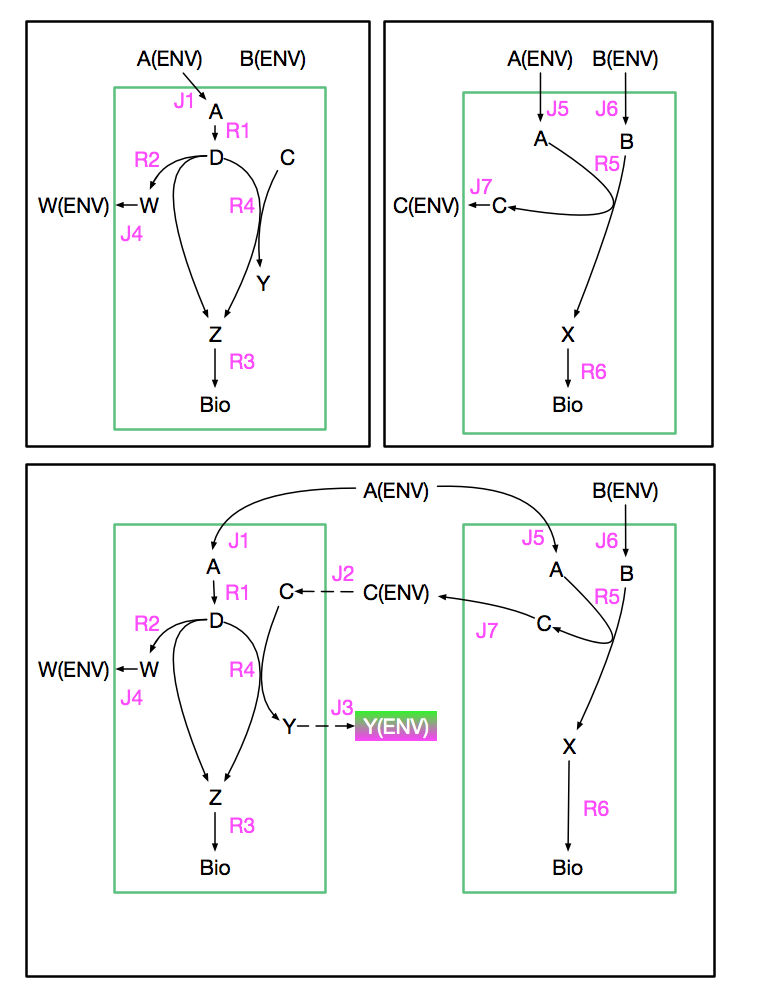
\includegraphics[width=0.35\textwidth]{figures/Organisms123.png}
\caption{Visualization of the co-culture formed by Organism 1 and Organism 2. Note the interaction between them by means of metabolite C, which Organism 1 processes to yield metabolites Y and Z.}
\label{Algo1Result1}
\end{figure}


\begin{comment}
\begin{multline*}
dA_{env} / dt = - Bio\\
dB_{env} / dt = - Bio\\
dC_{env} / dt = Bio\\
\end{multline*}
\end{comment}


Note that the nutrient uptake and metabolite secretion rates are given as functions of the biomass of the organism as well as the flux values. This is done to enforce the physically realistic condition that a larger organism possesses greater uptake potential while simultaneously requiring more of the necessary nutrients to survive and grow.

While the biomass in our model, denoted as $Bio$, could be considered an internal metabolite concentration (biomass is not shared between organisms in the extracellular medium), $dBio / dt$ is not included in the (internal) stoichiometric matrix $S$ because the steady-state condition $S \cdot v = 0$ does not apply to the biomass. Moreover, with increase in biomass, there eventually occurs creation of new microbial cells which we are not explicitly considering in our model. Thus increase in biomass is intimately tied to the concentration of metabolites in the extracellular medium. Hence, biomass itself is treated as an external metabolite. Indeed, it is desirable for biomass to increase, i.e. for growth to occur as much as possible within a time-step. The unique dynamics of $Bio$ are handled as a special case that will be further elaborated when discussing the modelling approach in detail. As shown in Fig \ref{Algo1Result1}, for all intents and purposes, in Organism 1, consider that $R_3$ alone contributes to the biomass and that $dBio / dt = R_3$. Likewise, in Organism 2, $dBio / dt = R_6$.

The bounds on the transport reactions are taken as the minimum of the Michaelis-Menten equations and maximum consumption rate per cell per time-step\cite{Chiu14}.
The Michaelis-Menten equations give the reaction rate for single-substrate reactions with the intermediate enzyme complex concentration fixed for short time-scales (quasi-steady-state assumption). Since flux-balance analysis is solely concerned with the fluxes that produce metabolic equilibrium (all uptakes and all secretions sum to zero), the Michaelis-Menten equations provide a limit for the rate of conversion at any given substrate concentration. The maximum consumption rate per cell per time-step considers the case wherein the environmental concentration of a nutrient is fully consumed by the organism(s) over the fixed time-step, $\Delta t$. Hence, the rate of uptake should be scaled proportionally to both the total biomass (each unit of biomass is allocated an equal amount of nutrient) and the size of time-step (to ensure a constant uptake rate throughout the entire interval).

Thus, for any uptake flux $J_x$ associated with metabolite $C_k$, $1 \leq k \leq M$, the lower bound at time $t$ is given as:
\[\large -min\{ \frac{V_m * C_k}{K_m + C_k}, \frac{C_k}{Bio * \Delta t}  \} \leq J_x \leq \infty \]

A lower bound instead of an upper bound is used to limit metabolite uptake from the growth medium, as uptake reactions are conventionally assumed to have a stoichiometric coefficient  of -1. The internal fluxes themselves remain unbounded.

% these go in the automata model not the cFBA representation of Chiu's model
\begin{comment}
\begin{multline*}
dA_{env} / dt = - 3 * Bio \\
dC_{env} / dt = 0\\
dW_{env} / dt = 2 * Bio \\
dY_{env} / dt = 0 \\
\end{multline*}

\begin{multline*}
dA_{env} / dt = -Bio \\
dC_{env} / dt = 0 \\
dW_{env} / dt = 0 \\
dY_{env} / dt = Bio \\
\end{multline*}
\end{comment}






\begin{comment}
To define these organisms as automata using the decomposed dynamics approach, the internal reactions can be discarded (as previously shown), leaving the organisms defined by:\\

\textbf{Organism 1}\\

\begin{multline*}
dBio / dt = R_3\\
dA_{env} / dt = -J_1 * Bio \\
dW_{env} / dt = J_4 * Bio \\
dC_{env} / dt = -J_2 * Bio \\
dY_{env} / dt = J_3 * Bio \\
\end{multline*}

\textbf{Organism 2}\\

\begin{multline*}
dBio / dt = R_6\\
dA_{env} / dt = -J_5 * Bio\\
dB_{env} / dt = -J_6 * Bio\\
dC_{env} / dt = J_7 * Bio\\
\end{multline*}

\end{comment}

\section{Flux-Based Modelling Approaches}

\subsection{Decomposing Steady-State Metabolism}


Dynamic FBA (dFBA) simulates the metabolism of an organism by solving for the steady-state fluxes that maximizes growth as the objective function, setting the resulting fluxes as constant for a sufficiently short time interval. The simulated growth flux is used to update the concentrations of biomass and metabolites in the extracellular medium at the end of the time step. The process is then iterated for the succeeding time-steps.
%($\Delta t = 0.02$ in Chiu's case)

% revisit this

While the dFBA algorithm clearly defines the trajectory of a continuous dynamical system, representing the underlying biological system as a hybrid automaton in its most generic form proves challenging. This is due to a) the inherent nondeterminism of the process, b) the difficulty of identifying the individual discrete states, and c) the algebraic constraints ($S \cdot v = 0$) on the flux values.

To elucidate further: the metabolite concentrations (internal or external) are governed by dynamics that depend on unknown flux values. Hybrid automata are able to represent systems with parameterized dynamics. Many model checkers for hybrid automata (among them, Flow*, HyPro) support verification on systems with parameterized dynamics -- given that the unknown parameters are at least bounded from one side. However, adding algebraic constraints to the parameters (like the steady-state requirement $S \cdot v = 0$, where $v$ is the flux vector) turns the dynamics of each state into a differential-algebraic system of equations (DAE). Differential-algebraic hybrid automata are significantly harder to reason about than regular hybrid automata, and while they have been used successfully to analyze biological systems, no general purpose model checker exists that can handle all biologically relevant cases where they occur. Thus, a different approach is desired -- one that maintains the generality of the biological system under consideration while falling nicely within standard hybrid automata representations.

% revisit this

While the final modelling approach fully generalizes any trajectory that can be computed by dFBA, handling the specific, deterministic case is first necessary to build the structural induction argument behind the general hybrid automaton. A hybrid automaton should be introduced that computes one trajectory for the microbe in question, as opposed to the desired approach, which uses nondeterminism to compute any biologically valid trajectory.

%For a specific microbial model within the dFBA formulation, the stochiometric matrices $S$ and $T$ and the bounds for each flux are known and not simulation-dependent. The size of the timestep, $\Delta t$, is determined before calculating any trajectory and is fixed for the duration of the simulation. Thus, it can be treated as a constant with respect to the dFBA in question. Within each time-step, the internal and external concentrations define the state of the system while the flux values parameterize the concentration dynamics. Thus, given a set of initial concentrations, the selection of the flux vector $v$ in each time-step is the only nondeterministic aspect of the trajectory.

The dFBA formulation for a specific organism induces a dynamical system given by the tuple $\mathbb{D} = (\overline{C}_{int}, \overline{C}_{ext}, S, T, v_{max}, v_{min}, \overline{C}_{0}, \Delta t, t_{max})$, where $\overline{C}_{int}$ and $\overline{C}_{ext}$ are vectors of the internal and external metabolite concentrations, $S$ and $T$ are matrices corresponding to the internal stoichiometry and uptake / secretion stoichiometry, $v_{max}$ and $v_{min}$ are the upper and lower bounds (respectively) for the vector of fluxes, $\overline{C}_{0}$ is the initial value vector for the metabolite concentrations ([$\overline{C}_{int}, \overline{C}_{ext}] = \overline{C}_{0}$ at $t = 0$), and $t_{max}$ is the end time of the trajectory. For a specific microbial model within the dFBA formulation, the stochiometric matrices $S$ and $T$ and the bounds for each flux are known and not simulation-dependent. The size of the timestep, $\Delta t$, is determined before calculating any trajectory and is fixed for the duration of the simulation. Thus, it can be treated as a constant with respect to the dFBA in question. The number of time steps is given by $n = \frac{t_{max}}{\Delta t}$. Within each time-step, $\overline{C}_{int}$ and $\overline{C}_{ext}$ define the state of the system while the flux values parameterize the concentration dynamics ($\frac{d\overline{C}_{int}}{dt}$, $\frac{d\overline{C}_{ext}}{dt}$). Thus, given a set of initial concentrations, the selection of the flux vector $v$ in each time-step is the only nondeterministic aspect of the trajectory.

It is to be noted that the objective function $G(v)$ that is usually given when describing dFBA is notably absent -- this is because the objective function often results in a nondeterministic selection of $v$ from several satisfactory options, so $G(v)$ itself is entirely arbitrary when precisely defining both the general dynamical system as well as a specific trajectory of the system. Trajectories are instead given directly by $\mathbb{T} = (\mathbb{D}, \overline{V} = [v_1, v_2, v_3..., v_n])$, where $n$ is the number of time steps and $\overline{V}$ is a sequence of flux vectors such that the flux vector $[\overline{V}]_k = v_k$ governs the concentration dynamics for the timestep ending at $k * \Delta t$. As shorthand, a specific trajectory of any $\mathbb{D}$ is denoted as $\mathbb{D}(\overline{V})$.
Using the previous formalism for dFBA, a hybrid automaton that exhibits the trajectory $\mathbb{D}(\overline{V})$ can be built by using the procedure in Algorithm \ref{Algo1}. Consider that for $\mathbb{D}(\overline{V})$, the continuous trajectory is divided into equal discrete intervals. The first interval of size $\Delta t$ has the concentration dynamics $d\overline{C}_{int}/dt = S * v$ and $d\overline{C}_{ext}/dt = T * v * Bio$ and parameterized by $[\overline{V}]_1 = v_1$. After time $\Delta t$ passes, a discrete ``switch" occurs and the dynamics are then parameterized by $[\overline{V}]_2 = v_2$. This switching, in practice, is forced by a ``clock" variable, $\tau$, where $d\tau / dt = 1$ and occurs upon $\tau > \Delta t$. $\tau$ is then reset to $0$. As this switching behavior only changes the parameterization of the dynamics, the concentrations themselves can be updated continuously throughout the process. Possessing a continuous state space with dynamics that ``switch" at fixed intervals, it should be obvious that $\mathbb{D}(\overline{V})$ can be easily represented as hybrid automata. As the dynamics of $Bio$ are not given in $\mathbb{D}$, consider $Bio$ to be constant and equal to 1.

It is known that any valid $v$ exists within the flux-cone induced by stoichiometry $S$ and the bounds $v_{max}$ and $v_{min}$. By definition, $v$ satisfies the equation $S \cdot v = 0$ which guarantees internal steady-state. Since the dynamics of the internal concentrations are given as $d\overline{C}_{int}/dt = S \cdot v$, $d\overline{C}_{int}/dt = 0$ for all values of $v$. Hence, $d\overline{C}_{int}/dt$ and $\overline{C}_{int}$ are not necessary to uniquely describe the state space of the system and can be discarded in the final model, leaving $X = \overline{C}_{ext} \cup \{\tau\}$ as the set of continuous variables. Accordingly, $\overline{C}_{0}$ should be restricted to only variables from $X$ as well.
\begin{algorithm*}[H]
\SetAlgoLined
 \textbf{Input:} The trajectory $\mathbb{T} = (\mathbb{D},\overline{V} = [v_1, v_2, v_3..., v_n]) = \mathbb{D}(\overline{V})$\;
\KwResult{Hybrid automaton $\mathbb{H}(\mathbb{D},\overline{V})$ that follows trajectory $\mathbb{D}(\overline{V})$\;}

 Initialize a hybrid automaton $\mathbb{H}$ where:\\
 \hspace*{10mm}Continuous variables $X = \overline{C}_{ext} \cup \{ \tau \}$;\ \\
  \hspace*{10mm}Discrete locations $L = \{ l_1, l_2, ..., l_n \}$;\ \\
  \hspace*{10mm}Initial condition  $I = (l_1,[\overline{C}_{0}, 0])$;\ \\
 \hspace*{10mm}Assign the dynamics of $l_1$ as:\\
                        \hspace*{20mm}$\frac{d\overline{C}_{ext}}{dt} = T \cdot v_1 * Bio$\;
                        \hspace*{20mm}$\frac{d\tau}{dt} = 1$\;

 \For{$i = 2; i <= n$}{
    Assign the dynamics of $l_i$ as follows:\\
                        \hspace*{10mm}$\frac{d\overline{C}_{ext}}{dt} = T \cdot v_i * Bio$\;
                        \hspace*{10mm}$\frac{d\tau}{dt} = 1$\;

    Add a forced transition from $l_{i-1}$ to $l_i$\ with guard condition $\tau > \Delta t$ and reset $\tau = 0$;
 }
 \textbf{Return} $\mathbb{H}$;\
 \caption{Transformation of dFBA trajectory $\mathbb{D}(\overline{V})$ to hybrid automaton $\mathbb{H}(\mathbb{D},\overline{V})$}
 \label{Algo1}
\end{algorithm*}

\begin{figure}[H]
\centering
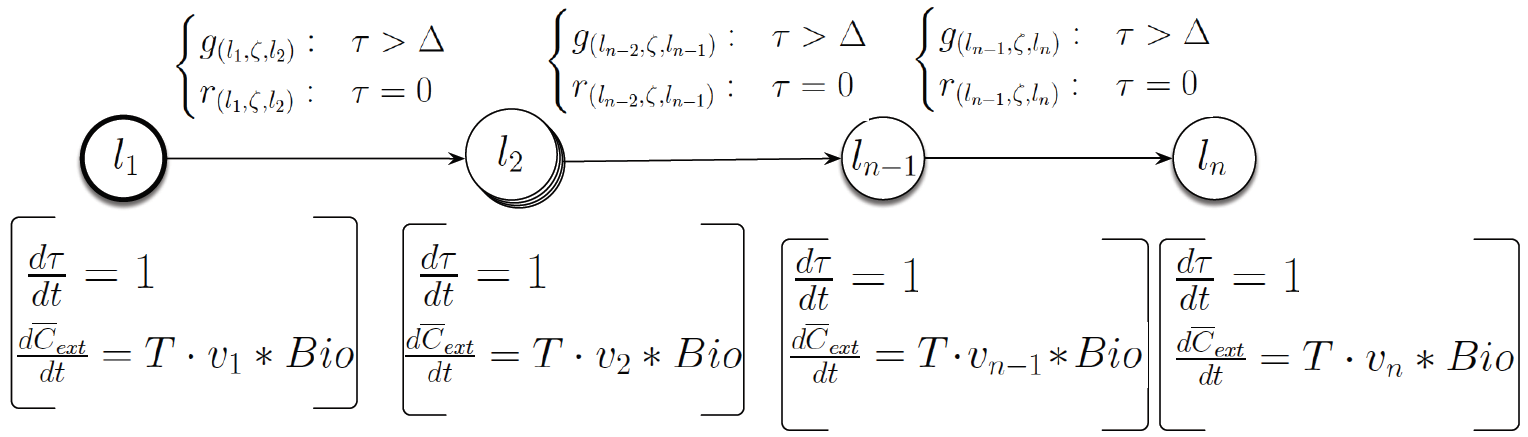
\includegraphics[width=1.0\textwidth]{figures/Algo1Result.png}
\caption{Visualization of $\mathbb{H}(\mathbb{D}, \overline{V})$ for an arbitrary $\mathbb{D}(\overline{V})$}
\label{Algo2Result2}
\end{figure}



The output automaton can be denoted by $\mathbb{H}(\mathbb{D}(\overline{V})) = \mathbb{H}(\mathbb{D}, \overline{V})$. During the construction process, the introduction of the clock variable, $\tau$ is the only explicit addition needed to represent $\mathbb{D}(\overline{V})$ as a hybrid automaton as shown in Fig \ref{Algo2Result2}. All other parameters come directly from $\mathbb{D}(\overline{V})$ itself.

While the construction $\mathbb{H}(\mathbb{D}, \overline{V})$ is a necessary step in designing a hybrid automaton that encapsulates $\mathbb{D}$, it is limited by its explicit dependence on $\overline{V}$. $\mathbb{D}$ can take any number of trajectories where $\overline{V}$ satisfies the stoichiometry and bounds. An automaton, $\mathbb{H}(\mathbb{D})$, is sought that can do the same that does not explicitly require $\overline{V}$ as a parameter for construction, initialization, and simulation. In particular, since $\overline{V}$ is chosen in a nondeterministic fashion, $\mathbb{H}(\mathbb{D})$ should be able to nondeterministically take any trajectory $\mathbb{D}(\overline{V})$.

To start, the procedure for constructing $\mathbb{H}(\mathbb{D})$ should be limited to the simplest case, $\overline{V} = [\overline{V}]_1 = v_1$, a singular constant flux, $v_1$ non-specified. Nondeterministic dynamics for an unspecified $v_1$ can be represented within the automaton by deconstructing the flux cone into its basic components. To recall, the flux cone is the convex polytope defined by the bounds and stoichiometry that contains all valid fluxes of the organism. Formally, the flux cone $\mathbb{F} \subset \mathbb{R}^N$, where $\mathbb{F} = \{v \; | S \cdot v = 0 \land v_{min} \leq v \leq v_{max} \}$. As the bounds themselves can be time-dependent, $\mathbb{F}$ is a differential inclusion. Denote the flux cone at time $t$ as $\mathbb{F}_t$. By ignoring the flux bounds and focusing only on the subspace defined by the stoichiometry, one receives $\mathbb{F}_{\emptyset} = \{v \; | S \cdot v = 0\}$, where $\forall t \geq 0, \mathbb{F}_t \subset \mathbb{F}_{\emptyset} \subset \mathbb{R}^N$. $\forall v, v \in \mathbb{F}_t \Rightarrow v \in \mathbb{F}_{\emptyset}$. The general solution of $S \cdot v = 0$  gives the linearly independent vectors $B = \{b_1, ..., b_n\}$, where $B$ form the bases of $F_{\emptyset}$. Thus, $\forall v \in \mathbb{F}_t$, $v = \sum^{n}_{i=1} b_i * k_i, k_i \in R$.

Using the previous representation of $v$, the automaton $\mathbb{H}(\mathbb{D})$ can be built for any $v_1$. Specifically, the equation $S \cdot v = 0$ is solved and the bases $B = \{b_1, ..., b_n\}$ are found. This procedure can be done using MATLAB or any standard numerical software package. Add $n$ discrete locations to the automaton, $L = \{ l_1, l_2, ..., l_n \}$, each location endowed with the same continuous variables and parameterized dynamics as the locations in $\mathbb{H}(\mathbb{D}, \overline{V})$. Each basis should then be ``assigned" to a corresponding location in the automaton, $b_1 \Rightarrow l_1, ..., b_n \Rightarrow l_n$, such that the basis vector parameterizes the dynamics of the location as shown in Fig \ref{Algo1Result2}. Add nondeterministic (unforced) transitions with guard condition ``true" from each location to the following location, where "following" is defined as the location $l_{j+1}$ for a location $l_j, j < n$. If $l_j = l_n$, there is no following location and thus no outgoing transition is added. In the same way as $\mathbb{H}(\mathbb{D},\overline{V})$, the dynamics of internal metabolites will always be steady-state, so $\overline{C}_{int}$ can be discarded from the final model, leaving $X = \overline{C}_{ext} \cup {\tau}$ as the set of continuous variables. Accordingly, $\overline{C}_{0}$ should be restricted to variables from $X$ as well. $S$ is initially needed to find the bases that describe the flux cone, but can be discarded in the final model as it only defines internal stoichiometry and dynamics.

Combining the parameterized dynamics with unforced transitions allow the dynamics of $\mathbb{H}(\mathbb{D},v_1)$ to be ``decomposed" generically such that the trajectory associated with any $v_1$ can be taken. However, the primary automaton of interest is a generic representation of $\mathbb{H}(\mathbb{D},\overline{V} = [v_1, v_2, ...,])$, $\overline{V}$ unspecified. This is accomplished by adding a nondeterministic (unforced) transition from $l_n$ back to $l_1$, with guard condition ``true". Hence, the transitions of the automaton form a cycle, where each ``forward" sequence of transitions ($l_1$ to $l_n$) possesses identical dynamic behavior to $\mathbb{H}(\mathbb{D},v_i)$. The transition from $l_n$ back to $l_1$ equates to the change in parameterization from some $v_i$ to $v_{i+1}$ within $\mathbb{H}(\mathbb{D},\overline{V})$. Hence, by ``unwrapping" $\mathbb{H}(\mathbb{D},\overline{V}=[v_1, v_2, ...,])$ into a sequence of automata [ $\mathbb{H}(\mathbb{D},v_1)$, $\mathbb{H}(\mathbb{D},v_2)$, ...] to be simulated in succession, then by ``decomposing" the dynamics of each $\mathbb{H}(\mathbb{D},v_i)$ into computationally equivalent trajectories composed of ``building block" dynamics, a generic automata $\mathbb{H}(\mathbb{D})$ for $\mathbb{H}(\mathbb{D},\overline{V})$ is built.


%The procedure to construct $\mathbb{H}(\mathbb{D})$ for any $v_1$ follows directly.








%Thus, for a specific dFBA (the stoichiometric matrix, the bounds on the fluxes,  a specific sequence of fluxes and The flux vector $v$




%and the corresponding hybrid automaton  the parameterized values of the form $S v = 0$ (where $v$ is the vector of all flux values)

%However, within the formalism of hybrid automata, selecting correct flux values with respect to the steady state is challenging because $S v = 0$ represents an algebraic relation, which, when combined with dynamics of the form $d\overline{X} / dt = \overline{C}$, turns the dynamics of the system into a differential-algebraic system of equations (DAE).

\begin{comment}
While it is possible to represent biological systems as DAEs and use solvers to compute their trajectories \cite{Kaplan:2009:MSMN}, systems of DAEs prove challenging to solve and specific DAEs often require specific techniques and approximations that are not easily generalizable to other systems, Hence, they aren't optimal as a general-case modeling paradigm for microbial metabolism.\\
\end{comment}


\begin{comment}
One way to circumvent the requirement of the stoichiometric matrix as an algebraic constraint while also preserving the constraints it represents is to decompose it into its most basic elements and embed that information into the dynamics of the model itself. This sounds challenging and poorly defined but can be accomplished easily using basic knowledge of linear algebra - specifically - we know that $S \cdot v = 0$ defines a flux cone, that all biologically feasible fluxes lie within the flux cone, and the subspace that the flux cone represents can be decomposed into its bases while preserving the structure of the space.

Since the flux cone defined by $S \cdot v = 0$ is equivalent to the null space of $S$, the bases of the null space can be found trivially using MATLAB or any other standard numerical software package.\\
\end{comment}


%Additionally, all metabolites must always be greater than equal or zero, so a flux value cannot be used that would assume that you have more of a metabolite than you presently do.

For the automata $H_1 = \mathbb{H}(\mathbb{D})$ and $H_2 = \mathbb{H}(\mathbb{D},\overline{V} = [v_1, v_2, ..., v_n])$, it must be shown that any trajectory achievable by $H_2$ is also achievable in $H_1$. For the purposes of simulation, the changes in the clock variable $\tau$, $d\tau / dt = 1$, should not be considered part of the ``trajectory." Indeed, $\tau$ is only necessary to force transitions within $H_2$. Thus, any trajectory $\mathbb{D}(\overline{V})$ taken by $H_2$ that results in a change in concentration of a metabolite must also produce that same change in concentration when $\mathbb{D}(\overline{V})$ is taken by $H_1$, for all metabolites.

In location $l_1$ of $H_2$, let the external metabolite $A$ with initial concentration $A_0$ be governed by the dynamics $\frac{dA}{dt} = F$, where $F$ is a linear combination of the transport fluxes $J_1, ..., J_h$. $\frac{dA}{dt}$ is specifically given by $[T \cdot v_1]_s$. %The length of each flux vector is the number of coluumns in the stoichiometric matrix that corresponds to the total number of fluxes in the organism including both internal reaction fluxes and transport fluxes at the boundary.

It is known that $\mathbb{F}_t$ defines the flux cone at time $t$, $\mathbb{F}_t \subset F_{\emptyset}$, and $v_1 \in \mathbb{F}_t$. The bases $\{ b_1, b_2, ..., b_n \}$ span the null space of $S$ and hence span $F_{\emptyset}$. Since $v_1 \in F_{\emptyset}$, $v_1 = \sum^{n}_{k=1} b_{k} * m_k, m_k \in R$.

It is also known that $v_1$ has the structure $[R_1, ...,  J_1, ..., J_h]$. Since $v_1 = \sum^{n}_{k=1} b_{k} * m_k$, for some $x, 1 \leq x \leq h$, $[v_1]_i = J_x = [\sum^{n}_{k=1} b_{k} * m_k]_i = \sum^{n}_{k=1} [b_{k}]_i * m_k$.  As $\frac{dA}{dt} = F = [T \cdot v_1]_s = \sum^h_{j=1} J_j * g_j$, each $J_j$ itself can be represented as a linear combination of bases that are then sub-indexed to the element corresponding to the $J_j$ flux. This is accomplished by transforming $[b_k]_i$ to an indexing of $j$. Specifically, $i = |v_1| - h + j$. Putting this together, $\frac{dA}{dt} = \sum^h_{j=1} J_j * g_j = \sum^h_{j=1} [\sum^{n}_{k=1} [b_{k}]_{\{|v_1|-h+j\}} * m_k] * g_j$. This rather un-intuitive expression can be simplified by making two observations: 1) the $m_k$ elements are the same for each iteration of the inner loop because $v_1$ is fixed, and 2) the indexed bases are the only terms that depend on $k$ and $j$, so the order of the loops can be reversed. This gives $\frac{dA}{dt} = \sum^{n}_{k=1} [\sum^h_{j=1} [b_{k}]_{\{|v_1|-h+j\}} * g_j] * m_k$. This can also be represented as $\frac{dA}{dt} = [T \cdot  \{\sum^{n}_{k=1} b_{k} * m_k\}]_s$.
As the initial condition of $A$ is $A_0$ and the dynamics $\frac{dA}{dt} = F$ are constant within $l_1$, the concentration of $A$ upon leaving $l_1$ at time $\Delta t$ (as forced by the transition from $l_1$ to $l_2$) is computed as $\int^{\Delta t}_{t = 0} F dt = A_0 + \Delta t * F$.\\

In location $l_1$ of $H_1$, the initial condition of $A$ is also $A_0$ but the dynamics are given by $\frac{dA}{dt} = [T \cdot b_{1}]_s$. Using the same steps as was done for $l_1$ of $H_2$, $[T \cdot b_{1}]_s =  \sum^h_{j=1} [b_1]_{\{|v_1|-h+j\}} * g_j$.
Thus, upon leaving $l_1$ at some arbitrary time (denoted $t_1$), the value of $A$ is given with $\int^{t_1}_{t = 0} \{ \sum^h_{j=1} [b_1]_{\{|v_1|-h+j\}} * g_j \} dt = A_0 + t_1 * \sum^h_{j=1} [b_1]_{\{|v_1|-h+j\}} * g_j$. For shorthand, denote the previous $A_0 + t_1 * \sum^h_{j=1} [b_1]_{\{|v_1|-h+j\}} * g_j$ as $A_1$. $A_1$ is the initial concentration of $A$ upon entering the location $l_2$ of $H_1$. Define $t_2$ as the elapsed time in the location $l_2$, or the time of transition $l_2 \Rightarrow l_3$ minus $t_1$. The dynamics of $A$ within $l_2$ are given as $\frac{dA}{dt} = [T \cdot b_{2}]_s$. The value of $A$ upon leaving $l_2$ is hence $\int^{t_2}_{t = 0} \{ \sum^h_{j=1} [b_2]_{\{|v_1|-h+j\}} * g_j \} dt = A_1 + t_2 * \sum^h_{j=1} [b_2]_{\{|v_1|-h+j\}} * g_j = A_0 + t_1 * \sum^h_{j=1} [b_1]_{\{|v_1|-h+j\}} * g_j + t_2 * \sum^h_{j=1} [b_2]_{\{|v_1|-h+j\}} * g_j$. Following the same steps, the concentration of $A$ upon leaving the location $l_n$ (completing a forward ``run" of the automaton) is given as $A_0 + t_1 * \sum^h_{j=1} [b_1]_{\{|v_1|-h+j\}} * g_j + t_2 * \sum^h_{j=1} [b_2]_{\{|v_1|-h+j\}} * g_j + ... + t_n * \sum^h_{j=1} [b_n]_{\{|v_1|-h+j\}} * g_j = \sum^{n}_{k=1} [\sum^h_{j=1} [b_{k}]_{\{|v_1|-h+j\}} * g_j] * t_k$.

From the previous, it becomes apparent that any change in $A$ produced in location $l_1$ from $H_2$ can be simulated in a forward ``run" of $H_1$:

$\int^{\Delta t}_{t = 0} F dt = A_0 + \Delta t * F =
A_0 + \Delta t * \sum^{n}_{k=1} [\sum^h_{j=1} [b_{k}]_{\{|v_1|-h+j\}} * g_j] * m_k = A_0 + \Delta t * m_1 * \sum^h_{j=1} [b_{1}]_{\{|v_1|-h+j\}} * g_j + \Delta t * m_2 * \sum^h_{j=1} [b_{2}]_{\{|v_1|-h+j\}} * g_j + ... + \Delta t * m_n * \sum^h_{j=1} [b_{n}]_{\{|v_1|-h+j\}} * g_j = A_0 + t_1 * \sum^h_{j=1} [b_{1}]_{\{|v_1|-h+j\}} * g_j + t_2 * \sum^h_{j=1} [b_{2}]_{\{|v_1|-h+j\}} * g_j + ... + t_n * \sum^h_{j=1} [b_{n}]_{\{|v_1|-h+j\}} * g_j$\\

This equivalence establishes that, to simulate $l_1$ of $H_2$ using $H_1$, the values $[t_1, t_2, ..., t_n] = [\Delta t * m_1, \Delta t * m_2, ..., \Delta t * m_n ]$ must be assigned. Hence, the total elapsed time needed to simulate the change in concentration is also found, where $\Delta t$ in $H_2$ becomes $\Delta t * \sum^n_{k=1} m_k$ in $H_1$. After leaving $l_n$ in $H_1$, $l_1$ is resumed and the process to simulate the dynamics of $l_2$ from $H_2$ can commence. $l_2$ is simulated by assigning $[t_1, t_2, ..., t_n] = [\Delta t * m'_1, \Delta t * m'_2, ..., \Delta t * m'_n ]$, where $v_2 = \sum^{n}_{k=1} b_{k} * m'_k$. This process is iterated to simulate the dynamics of $l_1, ..., l_{\frac{t_{max}}{\Delta t} }$ from $H_2$, where the original time $\Delta t * n$ needed to compute the trajectory $\mathbb{D}(\overline{V})$ directly through the dFBA framework becomes $\Delta t * \sum^{\frac{t_{max}}{\Delta t}}_{l=1} \sum^{n}_{k=1} m'^{(l-1)}_k$.


The previous procedure can be applied component-wise to every element of $\frac{d\overline{C}_{ext}}{dt}$, such that the result generalizes fully to all external concentration dynamics.\\ %to every element of $v_1$, such that the result fully holds for every flux $[R_1, ... ,J_j]$.


\begin{comment}
\textbf{Comment JFB: I am aware that in Chiu's model, he does not use a flux like F to determine uptake dynamics, but rather the uptake flux F times the biomass at the beginning of the timestep. Hence, the above for an uptake flux would in fact be $F * Bio_t$. However, biomass is assumed fixed within the timestep, and the update equation is applied upon exiting the timestep. So, the above still holds; the flux would just be scaled by $Bio_t$ which is fixed within the timestep (treated as a constant). In 4.4 I give the method to update biomass in $H_1$ the way it is handled in Chiu's model (reassignment to the variable $Bio$ upon the transition from $S_n$ to $S_1$.}\\
\end{comment}
%Since $F = \sum^{n}_{k=1} b_{k_i} * m_k$ for some specific set of $\{ m_1, ..., m_k \}$,
\begin{comment}
Thus, any change in the concentration of $A$ achieved by $H_1$ in $t$ time with associated flux $[\overline{V}]_{J_1}$ is achievable by $H_2$ in $(k_1 + k_2) * t$ time.\\

More generally, for a flux cone of $n$ bases instead of a fixed two, the change in the concentration of $A$ would be achieved in $\sum^{|B|}_{i=1} k_i * t$ time, where $|B|$ is the number of bases of the flux cone.\\

\end{comment}

\begin{comment}
However, this result only directly shows that uptake and secretion trajectories with constant flux can be broken down into smaller trajectories defined by basis fluxes. To fully encapsulate the power of dynamic FBA, we need to handle varying fluxes. The previous result is still applicable because dynamic FBA assumes that fluxes are changing over the time horizon, but are constant within a time step, and that the constant flux within the time-step is entirely responsible for the uptakes and secretions within that time-step. Specifically:\\

Assume that there exists a sequence of $n$ fluxes, all satisfying $S \cdot v = 0$, and all fluxes are fixed for an interval of $t$ time:\\

$v_1, v_2, v_3, ..., v_{n-1}, v_n$\\

It is known that each of these fluxes can be represented as a unique combination of the basis vectors of the flux cone (the general solution of $S * v = 0$). It's also known that the changes in concentrations within each time step, with respect to the fixed flux, are achievable by the system in a known amount of time using decomposition. Thus, the sequence of fluxes can decomposed into a sequence computable by the automata as:\\
However, the time step size is no longer constant; the time steps to simulate each flux are given as:\\

$\sum^{|B|}_{i=1} k_{i,1} * t, \sum^{|B|}_{i=1} k_{i,2} * t, \sum^{|B|}_{i=1} k_{i,3} * t, ..., \sum^{|B|}_{i=1} k_{i,n-1} * t, \sum^{|B|}_{i=1} k_{i,n} * t$\\

With the entire time to compute the sequence given by $t * \sum^n_{j=1}  \sum^{|B|}_{i=1} k_{i,j}$, as opposed to the $t * n$ needed to compute the sequence directly through the dynamic FBA framework.

\end{comment}
\begin{comment}
Starting off with a singular organism governed by simple dynamics, the dynamic FBA approach will be decomposed into its basic elements, and a reduction is constructed from a dynamic FBA computed on the organism to a sequence of transitions on an equivalent hybrid automata model of the organism. This automaton only computes steady-state fluxes with respect to the stoichiometry and encapsulates all trajectories computable by the dynamic FBA without loss of generality.
\end{comment}
\begin{algorithm*}[H]
\SetAlgoLined
 \textbf{Input:} A dFBA procedure formulated as the dynamical system $\mathbb{D} = (S, T, v_{max}, v_{min}, \overline{C}_{0}, \Delta t, t_{max})$\\
\KwResult{Hybrid automaton $\mathbb{H}(\mathbb{D})$}

 Solve $S \cdot v = 0$ to find the bases $B = \{b_1, ..., b_n\}$;\

 Initialize a hybrid automaton $\mathbb{H}$ where:\\

 \hspace*{10mm}Continuous variables $X = \overline{C}_{ext} \cup \{ \tau \}$;\ \\
  \hspace*{10mm}Discrete locations $L = \{ l_1, l_2, ..., l_n \}$;\ \\
  \hspace*{10mm}Initial condition  $I = (l_1,[\overline{C}_{0}, 0])$;\ \\

 \For{$i = 1; i <= |B|$}{
    Create location $l_i$ in $\mathbb{H}$\;
    Assign the dynamics of $l_i$ as follows:\\
                        \hspace*{10mm}$\frac{d\overline{C}_{ext}}{dt} = T \cdot b_i * Bio $\;
                        \hspace*{10mm}$\frac{d\tau}{dt} = 1$\;
    Add an unforced transition from location $l_{i-1}$ to location $l_i$\ with guard condition ``true" and label $\eta$;
 }

 Add an unforced transition from location $l_{n}$ to location $l_1$\ with guard condition ``true";\\

 \textbf{Return} $\mathbb{H}$;\\\
 \caption{Transformation of dynamical system $\mathbb{D}$ to hybrid automaton $\mathbb{H}(\mathbb{D})$}
\end{algorithm*}

\begin{figure}[H]
\centering
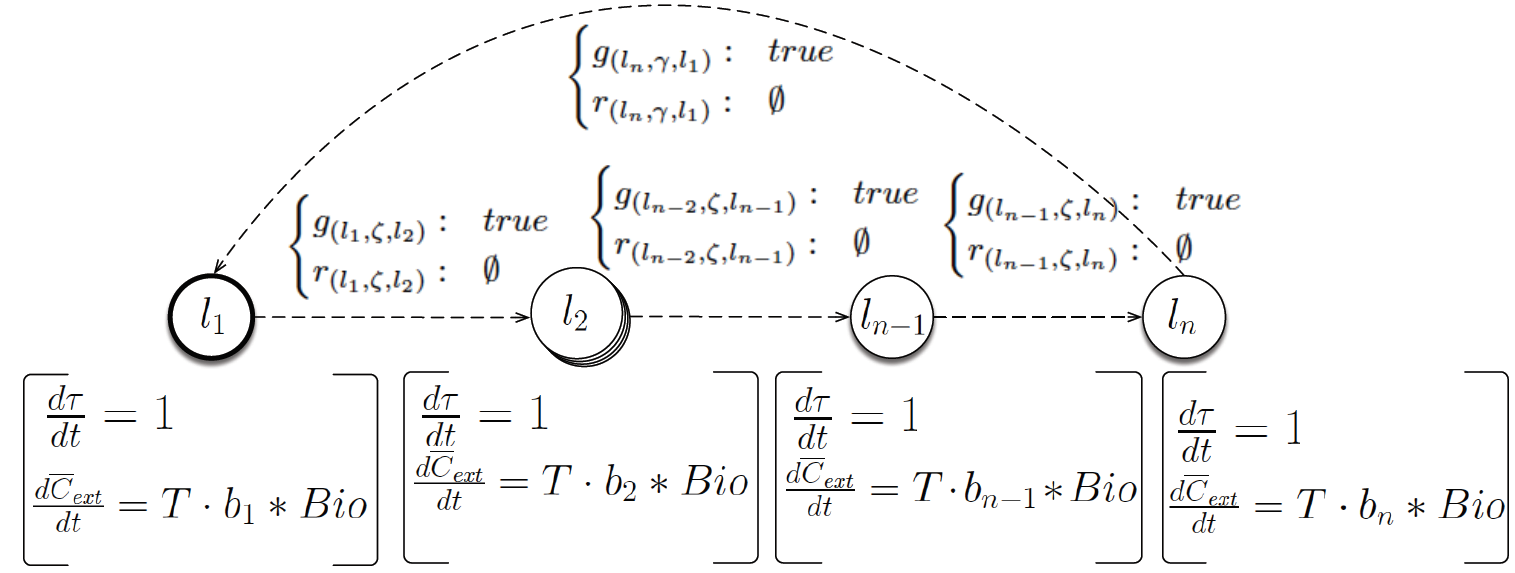
\includegraphics[width=1.0\textwidth]{figures/Algo2Result.png}
\caption{Visualization of $\mathbb{H}(\mathbb{D})$ for an arbitrary $\mathbb{D}$}
\label{Algo1Result2}
\end{figure}


\subsection{Representing Biological Growth}


While not technically a metabolite, the measure of biomass as a continuous variable $Bio$ is useful for many dFBA formulations as biomass is often used in assigning bounds and defining the objective function. The dynamics of biomass are usually formalized as monotonically increasing and a function of one or more ``internal" fluxes. While the dynamics could be given in the form $\frac{dBio}{dt} = v_i \cdot p$, $p \in R^{|v_i|}$, Chiu's model does not directly define $\frac{dBio}{dt}$. Instead, $Bio$ is updated at the end of every time-step $\Delta t$ as an exponential function of a singular flux value ($R_3$ for Organism 1).

This poses the question, then, of how to ``find" the selected $v_i$ (and by definition, $R_3$ or any other flux) upon the loop from $l_n$ back to $l_1$ in $H_1$.

%In $H_2$, this task is trial because $v_i$ is fixed and determined before the creation of the automata.

It is known that $v_i = \sum^{n}_{k=1} b_{k} * m_k, m_k \in R$. As the bases are fixed within $H_1$, $m_1, ..., m_n$ are the only degrees of freedom to determine the value of $v_i$. Furthermore, for each location $l_1, ..., l_n$ and the associated transition times $t_1, ..., t_n$, $[t_1, t_2, ..., t_n] = [\Delta t * m_1, \Delta t * m_2, ..., \Delta t * m_n ]$. %Hence, there is a direct relationship between the time $t_n$ and the constant $m_n$.

So, $v_i * \Delta t = \sum^{n}_{k=1} b_{k} * m_k * \Delta t  = \sum^{n}_{k=1} b_{k} * t_k$. As $\int^{t_k}_{t=0} b_k dt = b_{k} * t_k$, a vector of new variables with dimension $|v_i|$ should be added to $X$ (or more properly, $\overline{X}$, as $X$ itself is not vectorized), termed $\overline{Q}$, where, in each location $l_k$, $\frac{d\overline{Q}}{dt} = b_k$, and $\overline{Q} = 0$ at $t_0$ and upon the transition $l_n \Rightarrow l_1$. Before resetting from $l_n \Rightarrow l_1$, the sequence of transitions $l_1 \Rightarrow l_2, ..., l_{n} \Rightarrow l_1$ produces $\overline{Q} = \int^{t_1}_{t=0} b_1 dt + ... + \int^{t_n}_{t=0} b_n dt = \sum^n_{k=1} b_k * t_k = v_i * \Delta t$ and thus realizes the vector ``taken" in the forward ``run" of the automaton. Furthermore, upon the transition $l_n \Rightarrow l_1$, $Bio$ should be updated according to Chiu's model, as $Bio = Bio * e^{\Delta t * Bio_{agg}}$, where $Bio_{agg}$ is the sum of the individual fluxes that contribute to biomass accumulation. Since $\overline{Q} = v_i * \Delta t$ already includes the $\Delta t$ component, summing the necessary elements from $\overline{Q}$ is all that is required to produce $\Delta t * Bio_{agg}$. Create the vector $Bio_{sel}$ (where each element is either $0$ or $1$) such that $Bio_{sel} \cdot \overline{Q} = \Delta t * Bio_{agg}$. The reset can be reformulated as $Bio = Bio * e^{Bio_{sel} \cdot \overline{Q}}$. As $Bio$ is only updated upon the transition from $l_n \Rightarrow l_1$, $Bio$ becomes a step function when plotted with respect to $t$. Furthermore, because $Bio$ is constant within any forward ``run", the dynamics of the internal concentrations can be defined as $\frac{d\overline{C}_{ext}}{dt} = T \cdot b_i * Bio$, $Bio \neq 1$ while respecting the previously established equivalence between $H_1$ and $H_2$.

\begin{figure}[H]
\centering
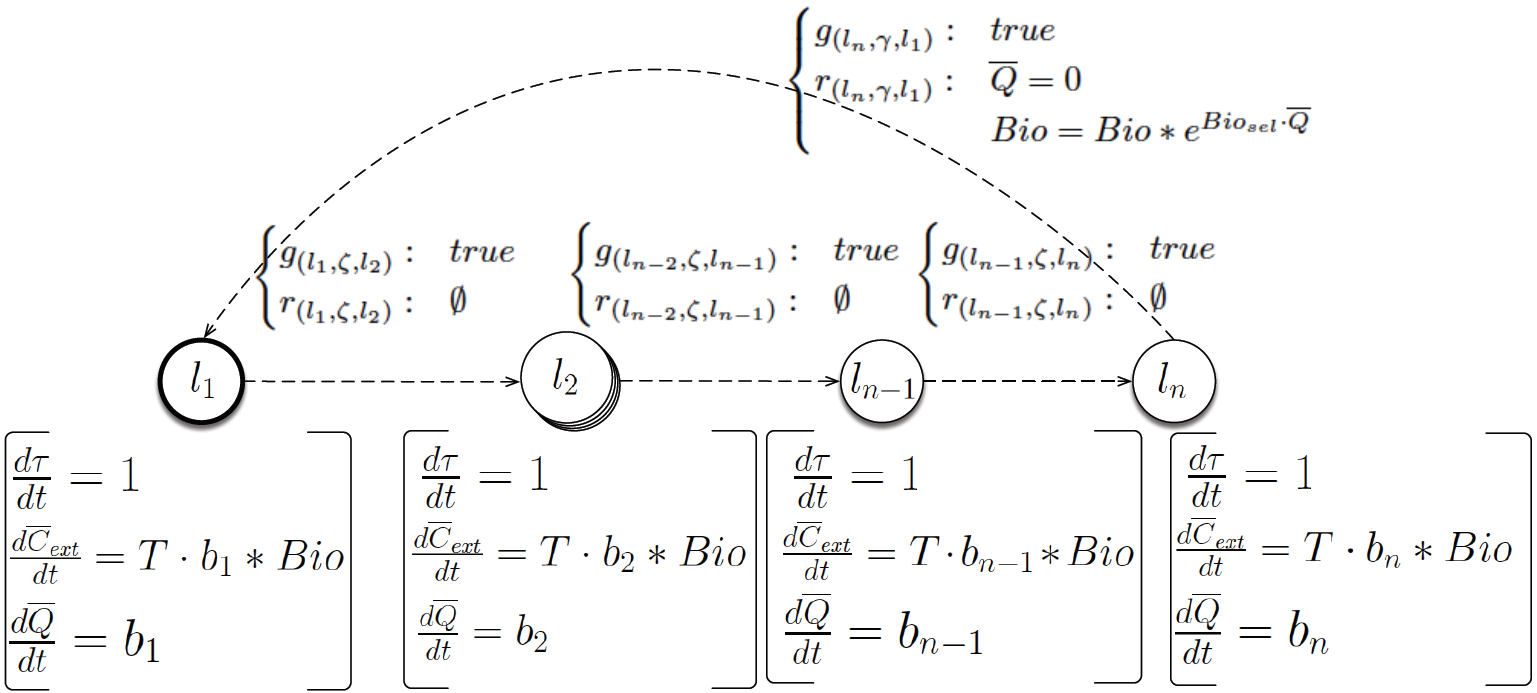
\includegraphics[width=1.0\textwidth]{figures/Algo2WithGrowth.png}
\caption{Output of Algorithm 2 with Biomass Accumulation}
\label{Organism2Automata}
\end{figure}

%Hence, an accumulator ``clock" variable, as was used to formalize bounds, also proves useful here.


%$Bio_{acc}$ has the form $\frac{dBio_{acc}}{dt} = \sum^j_{i=1} J_i * c_i$ and is reset as $Bio_{acc} = 0$ upon all transitions to $l_1$. Furthermore, upon those same transitions to $l_1$, $Bio$ is set as $Bio * e^{\Delta t * Bio_{acc}}$.



\subsection{Incorporating Flux Bounds with Decomposed Dynamics}

While the previous sections have established that, given a dFBA formulation $\mathbb{D}$, an automaton can be constructed to compute any arbitrary trajectory $\mathbb{D}(\overline{V})$, $\overline{V} = [v_1, v_2, ...]$ unspecified, an additional construction is necessary to fully represent the power of dFBA. Namely, $v_1, v_2, ...$ as previously defined are solutions to $S \cdot v = 0$ without considering the bounds $v_{min} \leq v \leq v_{max}$. Because the hybrid automata representation of $v$ was derived from $span \{b_1, b_2, b_3, ..., b_n\} =  \mathbb{F}_{\emptyset}$, $\exists v \in F_{\emptyset} \Rightarrow v \notin F_t$. Hence, the reachable set of $\mathbb{H}(\mathbb{D})$ is an overapproximation of the desired reachable set. The modified version of $\mathbb{H}(\mathbb{D)}$ which respects flux bounds shall be labeled $\mathbb{H}(\mathbb{D}, v_{max}, v_{min})$ = $\mathbb{H}(\mathbb{D, B})$.


%Since $\mathbb{H}(\mathbb{D})$ does not represent $[v_1, v_2, ...]$ directly, but rather as $v = \sum^{n}_{k=1} b_k * m_k $, linear combinations of the bases of $\mathbb{F}_{\emptyset}$, the scalar constants are the only true variables within the flux vector representation as the bases are fixed. Hence, the scalars must be constrained such that the upper and lower bounds of the resultant flux vector $v$ are not violated.

Specifically, for $v_{max}$ and some arbitrary external flux $J_x = [v]_i = [R_1, ..., J_1, ..., J_x, ..., J_h]$:\\

$ \sum^{n}_{k=1} m_k * b_k = v \leq v_{max}$

$ \sum^{n}_{k=1} m_k * b_k * \Delta t \leq v_{max} * \Delta t$

$ \sum^{n}_{k=1} \{m_k * \Delta t\} * b_k \leq v_{max} * \Delta t$


$\sum^{n}_{k=1} t_k * b_k \leq v_{max} * \Delta t$

$J_x * \Delta t = \sum^{n}_{k=1} t_k * [b_k]_i \leq [v_{max}]_i * \Delta t$\\

Invoking the $\overline{Q}$ variables, it is known that $\overline{Q} = 0$ upon the start of every ``run" $l_1 \Rightarrow l_2, ..., l_{n-1} \Rightarrow l_n$ and $\overline{Q} = v \Delta t$ at the end of the ``run", immediately before $l_n \Rightarrow l_1$. Thus, if the upper bound for $J_x$ is violated and $[v_{max}]_i * \Delta t < [v]_i * \Delta t$, there must exist some time $t_{\Phi}$ in some location $l_k$, $1 \leq k \leq n$, where $[\overline{Q}_{t_{\Phi} - dt}]_i < [v_{max}]_i * \Delta t < [\overline{Q}_{t_{\Phi} + dt}]_i$.

Thus, it becomes necessary to restrain $v * \Delta t$ (and by extension, $[v]_i * \Delta t$) by restricting $\overline{Q}$. This is done by adding transitions from each $l_k$, $1 \leq k \leq n$ to $l_1$, all labeled $\gamma$, whereupon $[\overline{Q}]_i > [v_{max}]_i * \Delta t$, the transition is forced to $l_1$ and the ``run" is prematurely terminated with the reset $\overline{Q} = 0$. Thus, the final value of $v * \Delta t$ that can be realized by any sequence of transitions $l_1 \Rightarrow l_2, ..., l_n \Rightarrow l_1$ with nondeterministically chosen transition times $t_1, ..., t_n$ is guaranteed to respect $v_{max}$. A ``premature" transition from $l_k \Rightarrow l_1$ at time $t_{\Phi}$ should still be considered a full ``run" and comprise a legitimate realization of $v * \Delta t$ because it is equivalent to the ``run" given by $t_1, ..., t_{\Phi}, 0, ..., 0$, with elapsed time of zero spent in each successor location.

Lower bounds from $v_{min}$ for any arbitrary $J_x$, $1 \leq x \leq h$ can be established likewise.


%upon performing the integration step of dFBA, $\int^{\Delta t}_{t = 0} J_x dt = \int^{\Delta t}_{t = 0} v[i] dt = F \Delta t + A_0$. The result is bounded as: $F \Delta t + A_0 = \sum^{n}_{k=1} t_k * b_k[i] \leq v_{max}[i] * \Delta t$. %In the last inequality, the only variable quantities are the $t_1, ..., t_{n}$ values. $B = \{ b_1, ..., b_n \}$, $v_{max}$, and $\Delta t$ are fixed with respect to $\mathbb{H}(\mathbb{D})$. Hence, the upper bound on $v$ is satisfied by selecting satisfactory $t_k$ values. However, individual $t_k$ values are not constrained -- it is a constraint on the weighted sum of the $t_k$ values.

%To handle this scenario, it is useful to consider the simpler case first. To constrain each individual $t_k$ (the amount of time spent in the location $l_k$), a clock would be assigned to each state of the automaton and a transition would be forced to either the next state or the first state when the maximum allowable time for $l_k$ has been reached. The value of this clock would be reset upon all transitions, including self-loops.

%If the total time of a "forward run" needed to be constrained (an upper bound on $\sum^{n}_{k=1} t_k$), a clock would be assigned to each state, but upon forward transitions (from a state $S_k$ to $S_{k+1}$), the clock value from the previous state would carry over -- only on the transition back to $S_1$ does the clock reset itself to zero. If the maximum clock value is reached at any state (too much time has been taken), a transition is forced to bring the system back to $S_1$.

%If a constraint on a weighted sum of the form $\sum^{n}_{k=1} c_k * t_k$ is desired, the previous approach is applicable with one modification - the clock assigned to each state $S_k$ ticks with a rate of $c_k$ instead of a rate of $1$. Clock values are still not reset at transitions except for the final transition back to $S_1$. Logically, the rate of the clock variable is assigned according to the ``contribution" from  $t_k$ to the total sum. If, for two states $\{S_k, S_{k+1} \}$, $t_{k} = t_{k+1}$ but $c_k > c_{k+1}$, each fraction of time spent in $S_k$ contributes more to $\sum^{n}_{k=1} c_k * t_k$ than the corresponding fraction of time in $S_{k+1}$.

%Thus, to account for all flux constraints, a "clock vector" should be added to the set of continuous variables $C$, where $\overline{Ck}$ has the same dimensionality as $v$. For each location $s_k$, $\frac{\overline{Ck}}{dt} = b_k$. The initial condition of $\overline{Ck}$ in $S_1$ is $\overline{0}$. Each location $l_1, ..., l_n$ is endowed with a transition back to $l_1$ with guard condition $L > \overline{Ck} \lor \overline{Ck} > U$ and reset $\overline{Ck} = \overline{0}$.

%The added constraints and associated transitions on the automata, $H$, are given as:

%These can be added to the example model, receiving:

\begin{figure}[H]
\centering
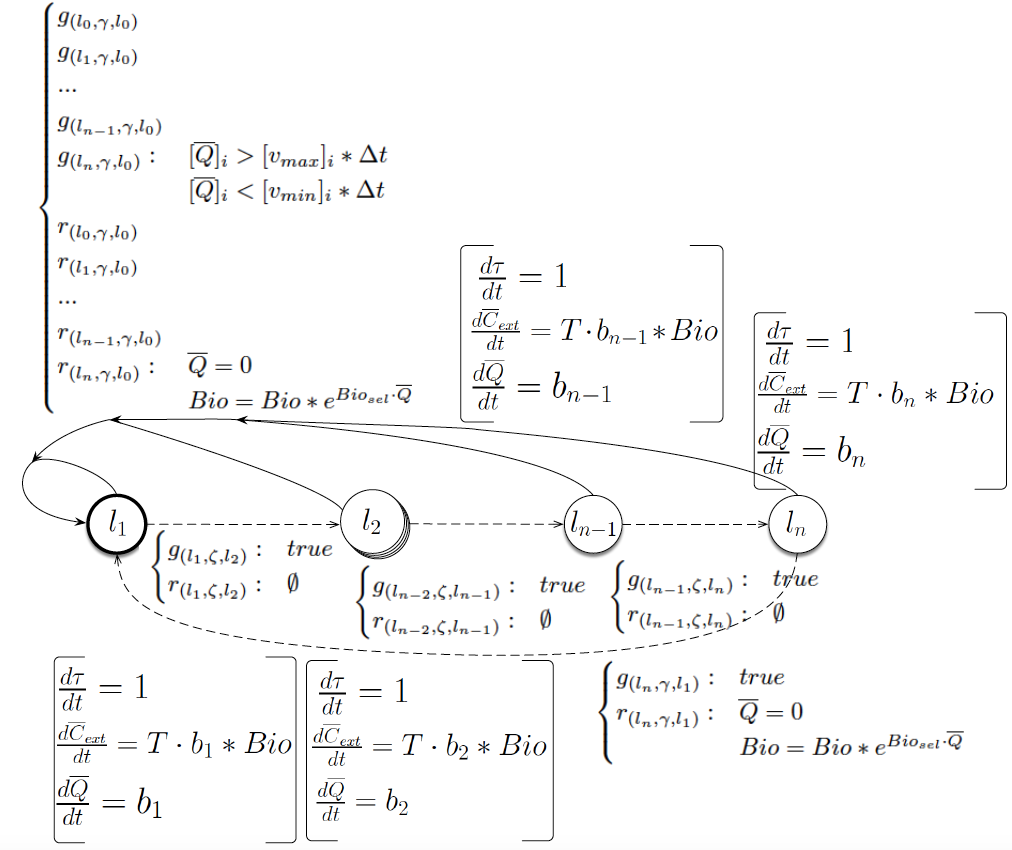
\includegraphics[width=1.0\textwidth]{figures/Algo2WithBounds.png}
% 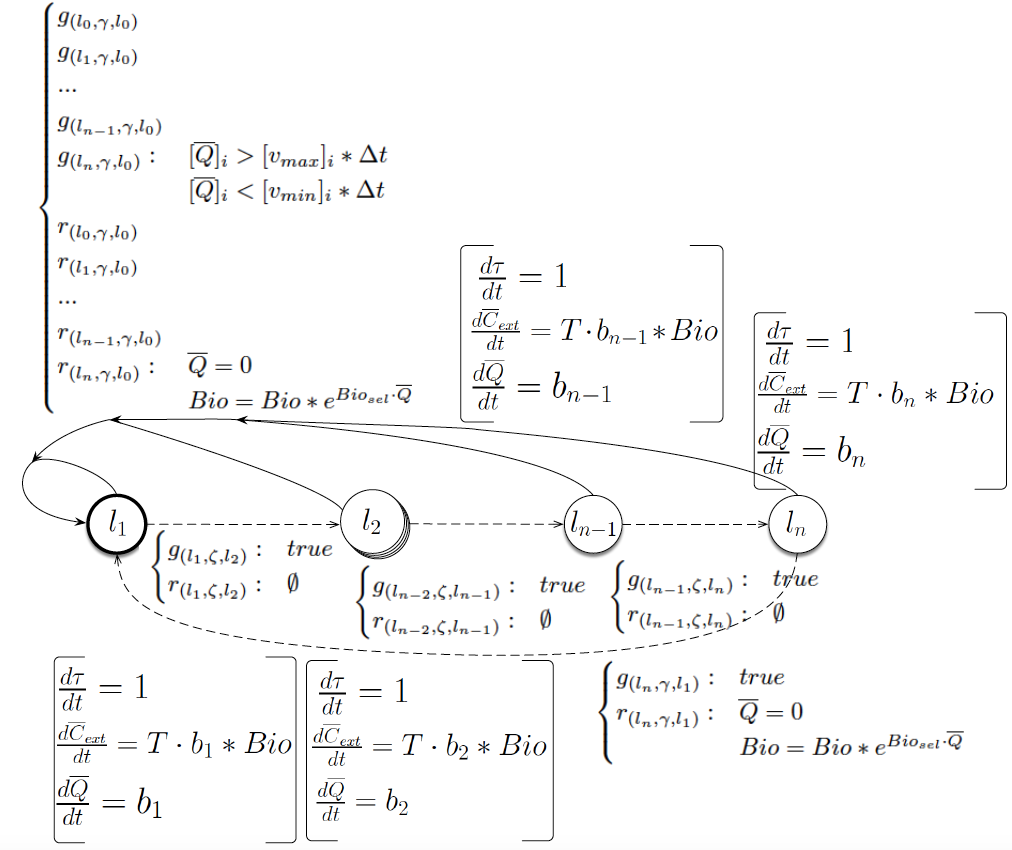
\includegraphics[width=0.57\textwidth]{figures/Algo2WithBounds.png}
\caption{Output of Algorithm 2 with Flux Bounds and Biomass Accumulation}
\label{Organism2Automata}
\end{figure}

\subsection{Replacing Nondeterminism with Deterministic Control}

The benefits to maintaining the nondeterministic formulation are plentiful. Particularly, when one in the early stages of research, the ability to explore all possible (while phenotypically sound) trajectories is necessary to understand the full metabolic capacity of a microbe. This is particularly useful when analyzing co-cultures, whose synergistic metabolism often exhibits nuanced interactions that can give rise to unexpected behavior over time. In addition, safety analysis can only be properly performed when considering the entire reachable set, or an overapproximation thereof. If only a handful of trajectories result in toxic metabolite secretion, it is preferable (and potentially much less costly) to reveal those scenarios during \textit{in silico} verification than run the risk of toxicity with live microbes. After-the-fact failure analysis also requires exhaustive state-space exploration, as the trajectory realized by the system did not equate to the trajectory predicted. Nevertheless, replacing the nondeterminism with a deterministic control mechanism is necessary if one wishes to simulate the realistic behavior of a microbe (e.g. what would be observed \textit{in vivo}) instead of performing theoretical analysis of the total metabolic capacity.

The nondeterministic transitions between a location $l_k$ and a successor location $l_{k+1}$ allow the automaton to indirectly represent any flux vector $v = \sum^{n}_{k=1} b_k * m_k$  by selecting transition times $[t_1, t_2, ..., t_n] = [\Delta t * m_1, \Delta t * m_2, ..., \Delta t * m_n ]$. %The generality of this approach is necessary to create an automaton with a reachable set that contains all possible trajectories, but a realistic biological system would choose only one trajectory from the set.
For each discrete time step of size $\Delta t$, which is represented in the automata by a forward ``run" from $l_1$ to $l_n$, a specific $v$ should be chosen according to some criterion. In other words, the \textit{unforced} transitions that emanate from each location $l_k$ to successor location $l_{k+1}$ (or $l_1$ in the case of $l_n$) would be replaced by \textit{forced} transitions with guard conditions of the most general form $G_{k}(\overline{C}_{ext}) > 0$. It is necessary to make the guard conditions explicit functions of the concentration levels while excluding time itself -- the microbe under consideration adjusts its behavior based on the concentrations in the environment, but it not capable of perceiving time nor engaging in temporal reasoning.

\begin{figure}[H]
\centering
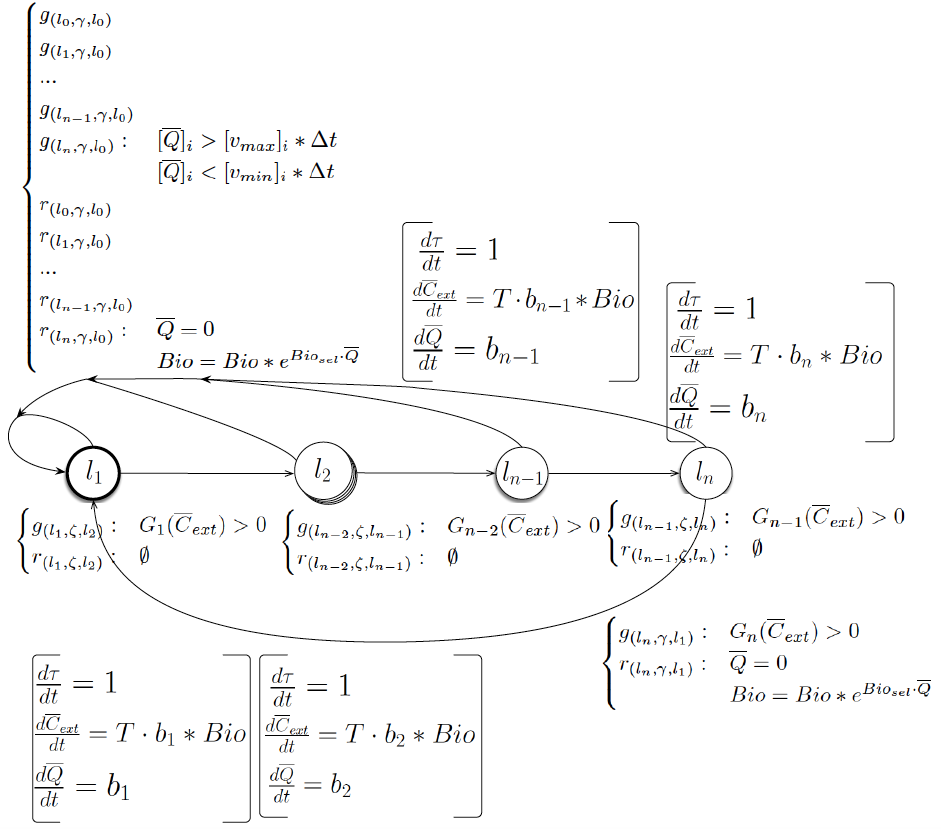
\includegraphics[width=1.0\textwidth]{figures/general-with-control.png}
% 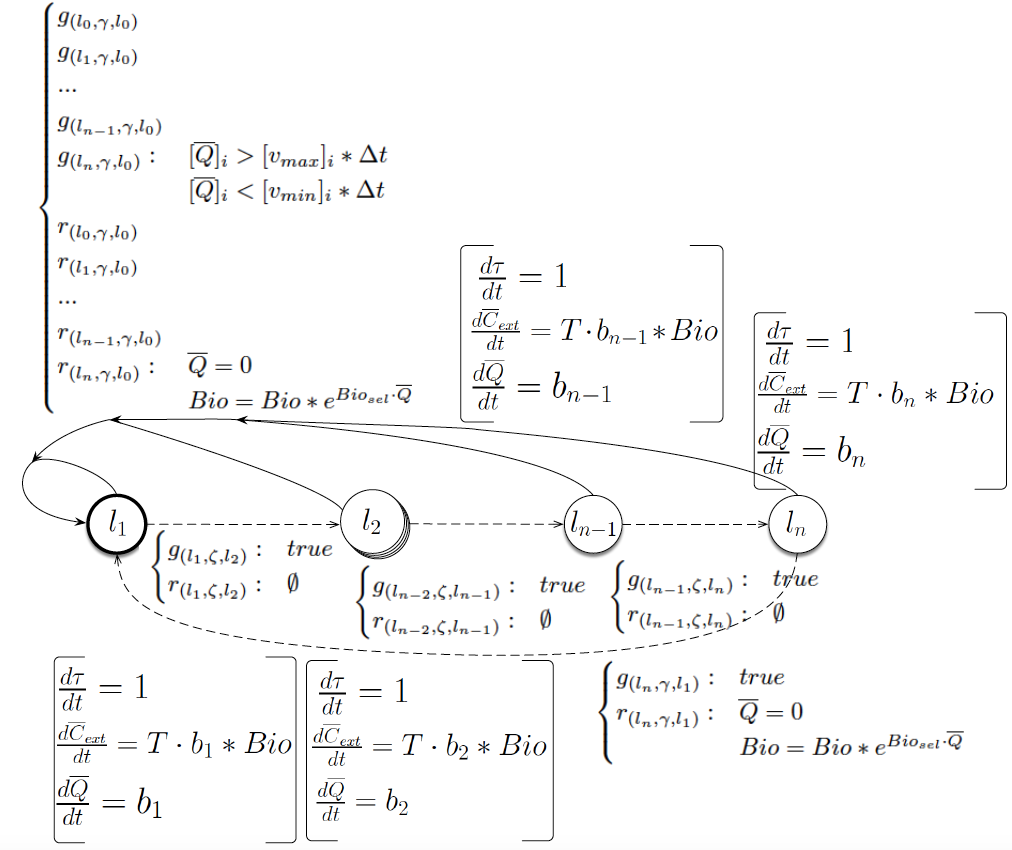
\includegraphics[width=0.57\textwidth]{figures/Algo2WithBounds.png}
\caption{Adapting the Automaton to use Deterministic Transitions}
\label{Organism2Automata}
\end{figure}

It has been shown that biologically relevant criteria for selecting fluxes include the optimal growth objective.
% find several other biolgically verified objective functions

Thus, control functions $G_{k}(\overline{C}_{ext})$, $1 \leq k \leq n$ should be chosen for each nondeterministic transition such that the resulting deterministic trajectory is optimal (or near-optimal) with respect to an objective function. Formally, this defines an optimal control problem on the automaton. This is a well-studied problem but solving it in the general case lies outside the direct scope of this work. However, the optimal control scenario is important to consider at a high level in order to build and represent a realistic microbial model. Specifically, in the case of Chiu's model organism, the control mechanism is already known, so the nondeterminism can be neatly replaced by a deterministic criterion without hassle. This is detailed further in Chapter \ref{chap:results}.



\subsection{Co-Culture as Composition of Automata}

There are two routes that can be taken to construct an automaton that represents a co-culture. The first is to model the locations, transitions and dynamics present in the co-culture directly, through careful inspection of the behavior of the combined system. This is time-consuming, prone to error, and potentially costly; if any change in co-culture composition is desired (say the user wants to replace one organism for another), the new co-culture must be modelled from the ground-up. The second option is to build a sound modelling framework for individual organisms (as has been done) and define a way to combine arbitrary individual automata into a co-culture automata. This can be achieved using an operation that will be called \textit{inner} (or \textit{dynamic}) \textit{composition}. This builds upon the conventional composition operation for hybrid automata by combining the dynamics for shared variables while respecting the dynamics for exclusive variables. In addition, it synchronizes transitions based on the event labels.

Composition for hybrid automata can be defined in several ways, so \textit{inner composition} will be used to refer to the one that has the following formal definition:

Define the two input automata $\mathbb{H}_1 = (X_1 \cdot L_1, I_1, \Sigma_1, Y_1, F_1, T_1, G_1, R_1)$ and $\mathbb{H}_2 = (X_2 \cdot L_2, I_2, \Sigma_2, Y_2, F_2, T_2, G_2, R_2)$. Let the sets $X_1$ and $X_2$ be vectorized as $\overline{X}_1$ and $\overline{X}_2$. Let the vector field $F_1$ be defined for all locations $l \in L_1$ as $d\overline{X}_1 / dt = \overline{f}_{l}(\overline{X}_1, t)$. Likewise, let the vector field $F_2$ be given as as $d\overline{X}_2 / dt = \overline{f}_{l}(\overline{X}_2, t)$ for all $l \in L_2$.

Construct a vector from $X_3 = X_1 \cup X_2$ and label it $\overline{X}_{3}$. Denote a new set of locations $L_3 = L_1 \cdot L_2$, wherein each $l \in L_3$ can be referenced as $(l_1 | l_2)$, $l_1 \in L_1$, $l_2 \in L_2$.  Endow each location $l \in L_3$ with the continuous state-space $X_{3}$. For each transition $(l_i, s, l_j) \in T_1$, where $s$ is either $\zeta$ or $s \notin \Sigma_2$, create transitions $\{ ((l_i | l_k), s, (l_j | l_k)) \}$, $1 \leq k \leq |L_2|$ between each pair of locations $(l_i| l_k), (l_j |l_k)  \in L_3$. Endow each transition with guard condition $G_{1}(t)$ and resets $R_{1}(t)$, where $t = (l_i, s, l_j)$.

Likewise, create transitions $\{ ((l_k | l_i), s, (l_k | l_j)) \}$, $1 \leq k \leq |L_1|$, between the pairs $(l_k | l_i), (l_k | l_j) \in L_3$ for each $(l_i, s, l_j) \in T_2$, where $s$ is either $\zeta$ or $s \notin \Sigma_1$. Endow each transition with guard condition $G_{2}(t)$ and resets $R_{2}(t)$, where $t = (l_i, s, l_j)$.

For $s \in \Sigma_1 \cap \Sigma_2$, $s \neq \zeta$, $(l_i, s, l_j) \in T_1$, $(l_u, s, l_v) \in T_2$, create transition $((l_i | l_u), s, (l_j | l_v))$ with guard condition $G_1((l_1, s, l_j)) \cup G_2((l_u, s, l_v))$ and resets $R_1((l_1, s, l_j)) \cup R_2((l_u, s, l_v))$. Add all of the newly created transitions to a set $T_3$ while adding the associated guards and resets to sets $G_3$ and $R_3$, respectively.

Create new sets $I_3 = I_1 \cup I_2$, $\Sigma_3 = \Sigma_1 \cup \Sigma_2$, $Y_3 = Y_1 \cup Y_2$.

For each location $(l_i | l_j) \in L_3$, define $d\overline{X}_3 / dt = [dx_1 /dt, dx_2 /dt, ..., dx_k /dt ,... dx_{|\overline{X_3}| } /dt] = \overline{f}_{l_i | l_j}(\overline{X_3}, t)$ as follows:

\[x_k / dt = \begin{cases}
      \overline{f}_{l_i}(\overline{X_1}, t) + \overline{f}_{l_j}(\overline{X_2}, t) & x_k \in X_1 \land x_k \in X_2 \\
      \overline{f}_{l_i}(\overline{X_1}, t) & x_k \in X_1 \land x_k \notin X_2 \\
      \overline{f}_{l_j}(\overline{X_2}, t) & x_k \notin X_1 \land x_k \in X_2
   \end{cases}
\],
where $l_i \in L_1, l_j \in L_2$. Label this new vector field over $L_3$ as $F_3$. Together, the automaton $\mathbb{H}_3 = (X_3 \cdot L_3, I_3, \Sigma_3, Y_3, F_3, T_3, G_3, R_3)$ is the result of the composition operation.

This operation can also be written, perhaps more elegantly, in vectorized form:

% rewrite the below
% s_i becomes l_i
% S` and S`` are sets of locations
For each $s_i \in S^{'}$, replace the continuous state-space of $X_1$ with the ``enhanced" state-space $X_3$. For each $x = X_1[k] \in X_1$, let $dx / dt = \overline{f}(\overline{X_1}, t)[k] = f_k(\overline{X_1}, t)$. For $x \in X_3$ where $x \notin X_1$, $dx / dt$ = 0. Hence, $\overline{X}_{s_i} /dt = \overline{f}(\overline{X_3}, t)$. Do the same for each $s_j \in S^{''}$ culuminating in $\overline{X}_{s_j} /dt = \overline{f}(\overline{X_3}, t)$. Hence $\overline{X}_{s_i| s_j} /dt$ is given directly by $\overline{X}_{s_i| s_j} /dt = \overline{X}_{s_i} /dt + \overline{X}_{s_j} /dt$.

\subsection{Algorithmically Assembling a Model}

A third and final algorithm can be formulated to assemble phenotypically-sound microbial models from the stoichiometry of the metabolic network. Unlike the preliminary model produced by Algorithm 2, these models include the flux bounds and growth mechanism as detailed in the previous sections. Thus, these models are a proper bisimulation of the dFBA models output by Algorithm 1 and do not contain trajectories that are not biologically sound.\\

\SetNlSty{texttt}{}{.}
\begin{algorithm*}[H]
\SetAlgoLined
\SetKwProg{ForInc}{for}{ do}{}

 \textbf{Input:} A dFBA procedure formulated as the dynamical system $\mathbb{D} = (S, T, v_{max}, v_{min}, \overline{C}_{0}, \Delta t, t_{max})$\\
\KwResult{Hybrid automaton $\mathbb{H}(\mathbb{D}, \mathbb{B})$}

 Solve $S \cdot v = 0$ to find the bases $B = \{b_1, ..., b_n\}$;\

 Initialize a hybrid automaton $\mathbb{H}$ where:\\

 \hspace*{10mm}Continuous variables $X = \overline{C}_{ext} \cup \overline{Q} \cup \{ \tau \}$;\ \\
  \hspace*{10mm}Discrete locations $L = \{ l_1, l_2, ..., l_n \}$;\ \\
  \hspace*{10mm}Initial condition  $I = (l_0, [\overline{C}_{ext}, \overline{Q}, \tau]) = (l_1,[\overline{C}_{0}, \overline{0}, 0])$;\ \\

 \ForInc{$i = 1; i <= n$}{
    Assign the dynamics of $l_i$ as follows:\\
                        \hspace*{10mm}$\frac{d\overline{C}_{ext}}{dt} = T \cdot b_i * Bio $\; \hspace*{10mm}$\frac{d\overline{Q}}{dt} = b_i $\;
                        \hspace*{10mm}$\frac{d\tau}{dt} = 1$\;
    Add an unforced transition from location $l_{i-1}$ to location $l_i$\ with guard condition ``true" and label $\eta$; \\
    \For{$j = 1; j <= |\overline{Q}|$}{
        Add a forced transition from location $l_i$ to location $l_1$ with guard condition $[\overline{Q}]_j > [v_{max}]_j * \Delta t$, label $\gamma$, and resets $r_{(l_i, \gamma, l_1)}: \{  Bio = Bio * e^{Bio_{sel} \cdot \overline{Q}}, \overline{Q} = \overline{0} \}$;
    }

 }

 \label{Algo3}
  \caption{Transformation of dynamical system $\mathbb{D}$ to hybrid automaton $\mathbb{H}(\mathbb{D}, \mathbb{B})$}
\end{algorithm*}

\newpage

\SetNlSty{texttt}{}{.}
\begin{algorithm*}[H]
\setcounter{AlgoLine}{15}
\SetAlgoLined
% This is to restore vline mode if you did not take the package as \usepackage[linesnumbered,ruled,vlined]{algorithm2e}
%This is to hide Begin keyword
\SetKwBlock{Begin}{}{end}
\Begin{
      \For{$j = 1; j <= |\overline{Q}|$}{
        Add a forced transition from location $l_i$ to location $l_1$ with guard condition $[\overline{Q}]_j < [v_{min}]_j * \Delta t$, label $\gamma$, and resets $r_{(l_i, \gamma, l_1)}: \{  Bio = Bio * e^{Bio_{sel} \cdot \overline{Q}}, \overline{Q} = \overline{0} \}$;
    }
 }

 Add an unforced transition from location $l_{n}$ to location $l_1$\ with guard condition ``true" and resets $r_{(l_i, \gamma, l_1)}: \{  Bio = Bio * e^{Bio_{sel} \cdot \overline{Q}}, \overline{Q} = \overline{0} \}$;\\

 \textbf{Return} $\mathbb{H}$;\\
\end{algorithm*}